\section{Method}
\label{sec:method}

\subsection{Overview}
A frozen detector supplies a mask \(M\), box \(B\), confidence \(s\), and decoder response \(p_i\) sampled on native image cell \(i\). We estimate occupancy on both sides of the contour (Section~\ref{sec:occupancy}), then test pairing at fixed signed counts (Section~\ref{sec:selection}) and allocation at fixed total count (Section~\ref{sec:variable-sign}). Detection identities, classes, boxes, and scores are fixed. A parallel control changes the write rule on one frozen Phoenix response (Fig.~\ref{fig:native-boundary}).

\begin{figure*}[!t]
\centering
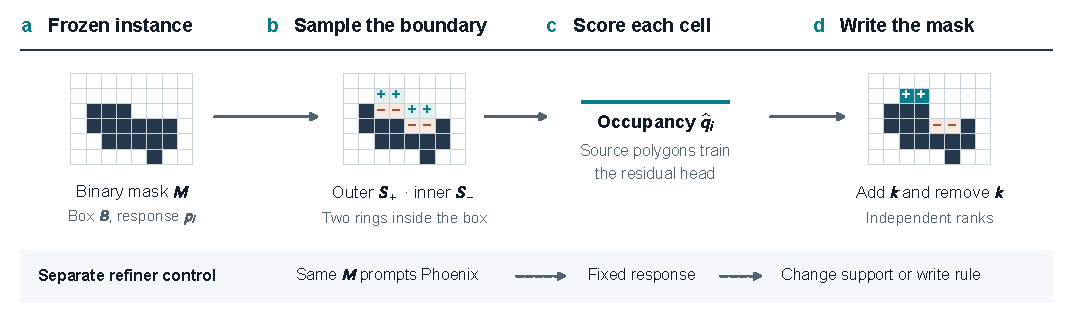
\includegraphics[width=\textwidth]{figures/matched_budget_pipeline.pdf}
\caption{The local pipeline fixes the detector output, samples native boundary cells, estimates their occupancy, and writes the selected edits. The lower lane compares writing rules on the same frozen refiner response.}
\label{fig:native-boundary}
\end{figure*}

\subsection{Native-Grid Sampling and Occupancy}
\label{sec:occupancy}
Let \(\Omega\) be the decoded \(W\)-by-\(H\) grid. Cell \(i=(x,y)\) covers \(C_i=[x,x+1)\times[y,y+1)\), and \(M_i=\mathbf{1}\{i\in M\}\). For \(B=[x_1,x_2)\times[y_1,y_2)\), inclusion is tested on the integer indices \(x,y\). For a response plane of width \(W_m\), native column \(x\) maps to \((x+\tfrac12)W_m/W-\tfrac12\), with the corresponding height map. D-FINE supplies a \(160\times160\) uncropped sigmoid plane. Its CPU feature path rounds the plane to FP16, bilinearly interpolates in FP32 with edge clamping, and rounds the sample to FP16. RF-DETR applies sigmoid after interpolating its logits. The saved binary mask determines the edit sign, including at sites where the sampled response and native binary decision differ.

For \(32\le |M|<1024\), use square \(3\times3\) dilation \(\delta\) and erosion \(\varepsilon\) with zero exterior. The two-layer support pools are
\begin{equation}
\begin{aligned}
\mathcal B_+&=(\delta^2(M)\setminus M)\cap B\cap\Omega,\\
\mathcal B_-&=(M\setminus\varepsilon^2(M))\cap B\cap\Omega.
\end{aligned}
\label{eq:native-bands}
\end{equation}
Layer \(\ell_i\) is one in the first ring and two in the second. We retain the first \(n=\min(32,|\mathcal B_+|,|\mathcal B_-|)\) sites on each side in ascending order of \((|p_i-\tfrac12|,yW+x)\), giving \(S_+\) and \(S_-\). Masks outside the area range or with \(n=0\) retain their original shape. Fig.~\ref{fig:occupancy-stage} shows the native support and supervision.

\begin{figure}[t]
\centering
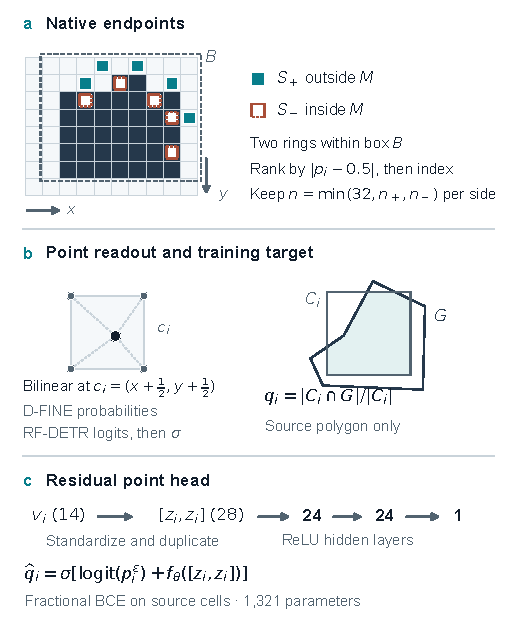
\includegraphics[width=\columnwidth]{figures/method_native_occupancy.pdf}
\caption{The two native rings supply candidate additions and removals. The reference polygon supplies fractional cell coverage during training, and the point head corrects the decoder response with a learned logit residual.}
\label{fig:occupancy-stage}
\end{figure}

A source-training candidate supplies supervision if it has a nonignored native COCO match at the raster IoU threshold of \(0.50\) and a valid reference polygon \(G\). Its target is the area fraction
\begin{equation}
q_i=|C_i\cap G|/|C_i| .
\label{eq:fractional-target}
\end{equation}
The 14 inputs comprise response and membership, boundary geometry, box-relative and candidate descriptors, and local appearance. In implementation order, the vector is
\begin{equation}
\begin{aligned}
v_i=\big(&p_i,M_i,\ell_i,d_i,\bar x_i,\bar y_i,\nu,\eta,s,\\
        &L_i,\bar L_3(i),\bar L_5(i),\Delta_x L_i,\Delta_y L_i\big)^\top .
\end{aligned}
\label{eq:endpoint-features}
\end{equation}
Here \(d_i\) is Euclidean distance to the nearest opposite-class cell, with background outside the grid. The box coordinates are \(\bar x_i=(x-x_1)/(x_2-x_1)\) and \(\bar y_i=(y-y_1)/(y_2-y_1)\). Area descriptors are \(\nu=\log_2|M|\) and \(\eta=|M|/|B\cap\Omega|\), with the latter denominator counting native box indices. The decoded red, green, and blue values \(c_i^R,c_i^G,c_i^B\) give \(L_i=(0.299c_i^R+0.587c_i^G+0.114c_i^B)/255\). With edge replication, the local mean and horizontal difference are
\begin{equation}
\begin{aligned}
\bar L_w(i)&=w^{-2}\!\!\sum_{j\in\mathcal N_w(i)}L_j,\\
\Delta_x L_i&=(L_{x+1,y}-L_{x-1,y})/2 ,
\end{aligned}
\label{eq:appearance-features}
\end{equation}
where \(\mathcal N_w(i)\) is the centered \(w\times w\) neighborhood and \(\Delta_y L_i\) uses the analogous row difference.

In the single-reference head, \(E_j\) averages training endpoints in source group \(j\). The training-only standardization uses
\begin{equation}
\mu=J^{-1}\sum_{j=1}^{J}E_j[v],\quad
\sigma_v^2=J^{-1}\sum_{j=1}^{J}E_j[v^2]-\mu^2 .
\label{eq:group-standardization}
\end{equation}
We clip negative roundoff in the variance to zero and use unit scale when the resulting scale is below \(10^{-12}\). For \(z_i=(v_i-\mu)/\sigma_v\) and \(p_i^\epsilon=\operatorname{clip}(p_i,10^{-4},1-10^{-4})\), the prediction is
\begin{equation}
\widehat q_i=\operatorname{sigmoid}
 \big(\operatorname{logit}(p_i^\epsilon)+f_\theta([z_i,z_i])\big).
\label{eq:occupancy-head}
\end{equation}
The two-hidden-layer ReLU head maps \(28\to24\to24\to1\) with 1,321 parameters. Input duplication matches the capacity of the partner-context control. The final affine layer starts at zero, so initial predictions follow the clipped response. Each batch samples groups uniformly and takes a pair within each sampled group. With \(m=64\), the loss averages both sides.
\begin{equation}
\mathcal L_{\rm occ}=\frac{1}{2m}\sum_{j=1}^{m}
  \left[\operatorname{BCE}(q_{a_j},\widehat q_{a_j})+
        \operatorname{BCE}(q_{d_j},\widehat q_{d_j})\right].
\label{eq:occ-loss}
\end{equation}
Here \(\operatorname{BCE}(y,p)=-y\log p-(1-y)\log(1-p)\). AdamW runs for 200 updates with learning rate \(0.002\) and weight decay \(0.01\). Each FIT109 development fold excludes its held source prefixes from fitting and standardization. Transfer freezes the weights and scaling obtained from all FIT109.

\subsection{Endpoint Selection at Equal Signed Counts}
\label{sec:selection}
List \(S_+\) and \(S_-\) in row-major order as \(a_j\) and \(d_j\). Fixed pairing first solves
\begin{equation}
\pi^\star\in\arg\min_{\pi\in\mathfrak S_n}
  \sum_{j=1}^n\|a_j-d_{\pi(j)}\|_2^2 .
\label{eq:fixed-assignment}
\end{equation}
We keep the assignment returned by SciPy on this integer cost matrix. The fixed writer ranks the pair gains \(\widehat q_{a_j}-\widehat q_{d_{\pi^\star(j)}}\) in descending order with addition-row ties. It keeps positive gains up to \(K=\min(8,\lfloor |M|/10\rfloor,n)\). Denote the realized count by \(k\), including the case \(k=0\). At this same count the independent writer solves
\begin{equation}
\max_{\substack{A\subseteq S_+,\,D\subseteq S_-\\ |A|=|D|=k}}
  \left(\sum_{i\in A}\widehat q_i-\sum_{i\in D}\widehat q_i\right).
\label{eq:independent-estimated-gain}
\end{equation}
This selects the highest occupancies on the addition side and the lowest on the removal side, breaking ties by the original pairing-row ordinal. The natural-count comparison retains positive gains under the independent ranks up to \(K\). Figure~\ref{fig:selection-stage} illustrates the fixed-count comparison.

The bounded writer tests whether reassigning partners accounts for the gain while preserving the maximum individual displacement. For \(k>0\), let \(H_{\rm fix}\) contain the \(k\) accepted pairs of the distance-first writer. Set \(\rho^2=\max_{(a,d)\in H_{\rm fix}}\|a-d\|_2^2\). On the graph with edges satisfying \(\|a-d\|_2^2\le\rho^2\), the bounded writer solves
\begin{equation}
\max_{\substack{H\ \text{matching}\\ |H|=k}}
\sum_{(a,d)\in H}(\widehat q_a-\widehat q_d).
\label{eq:bounded-endpoint-matching}
\end{equation}
Each site appears at most once. If the independent endpoint sets admit such a matching, we use them. Otherwise we solve \eqref{eq:bounded-endpoint-matching} by unit-capacity minimum-cost flow. The cap applies to individual edges. Total displacement and connectivity can vary. The three feasible sets are nested, so the estimated gains are ordered from distance-first to bounded to independent.

\begin{figure*}[!t]
\centering
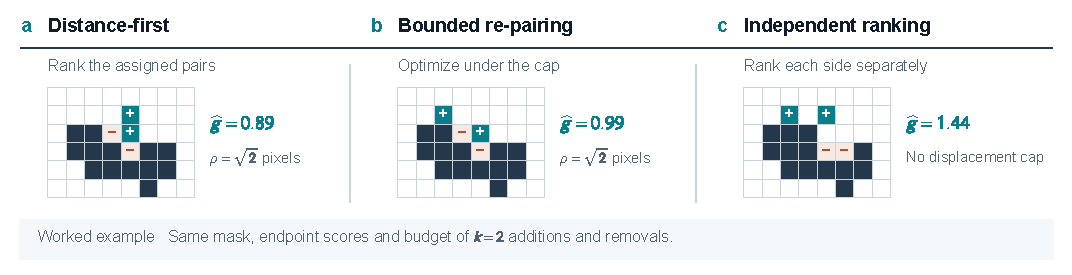
\includegraphics[width=\textwidth]{figures/method_bounded_selection.pdf}
\caption{Three writers at the same signed counts. The bounded writer re-pairs sites under the inherited displacement cap. Independent selection removes this cap. The worked example marks the two additions and removals in each output. The value \(\widehat g\) is the estimated intersection gain.}
\label{fig:selection-stage}
\end{figure*}

Write \(P=|M|\), \(T=|G|\), \(I=|M\cap G|\), and \(U=P+T-I\) in native area units. For the edited mask \(W'=(M\setminus D)\cup A\), its area change \(d\) and exact intersection change \(g\) are
\begin{equation}
d=|A|-|D|,\qquad
g=\sum_{i\in A}q_i-\sum_{i\in D}q_i .
\label{eq:intersect-changes}
\end{equation}
The new mask has area \(P+d\), intersection \(I+g\), and union \(U+d-g\). Subtracting \(I/U\) gives
\begin{equation}
\Delta\mathrm{IoU}=\frac{(P+T)g-Id}{U(U+d-g)} .
\label{eq:variable-area}
\end{equation}
For equal signed counts, \(d=0\) and IoU strictly increases with \(g\). Let \(g_{\rm pair}\) and \(g_{\rm ind}\) be the true gains under distance-first and independent selection. Common edits cancel, leaving the symmetric difference \(\mathcal D\) of the written sites. Optimality under the estimated gains gives
\begin{equation}
g_{\rm pair}-g_{\rm ind}
 \le \sum_{i\in\mathcal D}|\widehat q_i-q_i|
 \le 4k\max_{i\in S_+\cup S_-}|\widehat q_i-q_i| .
\label{eq:selection-error}
\end{equation}
Occupancy errors can reverse the ordering for a fixed match. COCO can also reassign matches at each IoU threshold.

\subsection{Dual-Reference Allocation at a Fixed Total Count}
\label{sec:variable-sign}
For the D-FINE allocation comparison, dynamic attraction supplies the candidate count \(k_s\), and static attraction at that count supplies the incumbent action \(S=(A_S,D_S)\) (Section~\ref{sec:phoenix}). A separate 1,346-parameter head takes the duplicated 14-dimensional feature vector and uses two 24-unit hidden layers. It applies the residual form in \eqref{eq:occupancy-head} with a separate final output for each reference. Training uses binary raster targets from paired author instances with mutual raster IoU at least \(0.50\) and the same native detection match. Eligible candidates have \(n>k_s>0\) and at least one nonidentity action. The 848 qualifying candidates span 447 images in 439 decoded groups. The head uses training-only group, image, candidate, and endpoint weighting for scaling. Each of 1,000 AdamW updates samples 64 candidates through groups and images, using a learning rate of 0.002 and weight decay of 0.01. BCE averages the signed endpoints and both references within a candidate, then weights each sampled candidate equally. At each seed all allocation policies use the same head.

Let \(E=S_+\cup S_-\) and \(\widehat q_{ir}\) denote occupancy under reference \(r\). Outside \(E\) the approximation takes the native labels as deterministic. Thus,
\begin{equation}
\begin{aligned}
\widehat T_r&=|M\setminus E|+\sum_{i\in E}\widehat q_{ir},\\
\widehat I_{r0}&=|M\setminus E|+\sum_{i\in E\cap M}\widehat q_{ir}.
\end{aligned}
\label{eq:dual-area-proxy}
\end{equation}
With \(g_r=\sum_{i\in A}\widehat q_{ir}-\sum_{i\in D}\widehat q_{ir}\) and \(d=|A|-|D|\), the ratio of expected intersection to expected union is
\begin{equation}
\widehat f_r(A,D)=
\frac{\widehat I_{r0}+g_r}{P+d+\widehat T_r-\widehat I_{r0}-g_r}.
\label{eq:dual-est-iou}
\end{equation}
Write \(a=|A|\) and \(b=|D|=2k_s-a\). The feasible integer range is \(\max(0,2k_s-n)\le a\le\min(n,2k_s)\). For \(\lambda\in\{0,0.1,\ldots,1\}\), we rank the two sides by \(\lambda\widehat q_{i1}+(1-\lambda)\widehat q_{i2}\), descending for additions and ascending for removals. Endpoint ties follow the archived order. For each split, we cross the first \(a\) and \(b\) entries of the corresponding side orders across all mixtures and add the incumbent side where its count permits. This gives a finite menu of action pairs, with score
\begin{equation}
J(A,D)=\min_{r\in\{1,2\}}\left[\widehat f_r(A,D)-\widehat f_r(S)\right].
\label{eq:dual-maximin}
\end{equation}
The incumbent is evaluated first. Splits follow increasing \(|a-k_s|\) and then \(a\), with ties retaining the first action. The equal control admits only \(a=k_s\), and a sensitivity admits feasible \(a\in\{k_s-1,k_s,k_s+1\}\). The proposal rule and total \(2k_s\) flips are shared (Fig.~\ref{fig:signed-allocation}). Alternative full-menu objectives use mean IoU gain or minimum raw-intersection gain.

\begin{figure*}[!t]
\centering
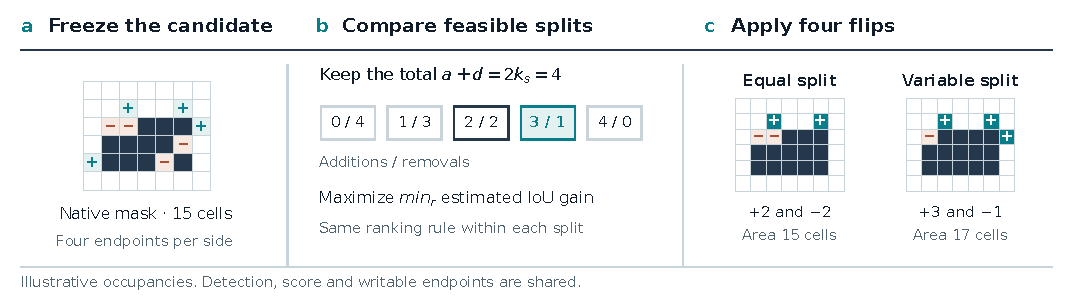
\includegraphics[width=\textwidth]{figures/method_signed_allocation.pdf}
\caption{Illustrative allocation at a fixed total of four flips. The equal split adds two cells and removes two. The maximin choice in this example adds three and removes one, changing the final area at the same total count.}
\label{fig:signed-allocation}
\end{figure*}

Equation~\eqref{eq:dual-est-iou} uses the reciprocal of the mean union, as in the RankIoU approximation~\cite{rankrma}. To assess this approximation on the same menu, we also compute the exact expectation under an independent Bernoulli model for the uncertain cells of each reference. The overlap \(I_r(W')\) and foreground count \(Z_r(W')\) outside \(W'\) involve disjoint sites. Their independence gives
\begin{equation}
\widehat f^{\rm E}_r(W')=\mathbb E[I_r(W')]\,
             \mathbb E[(|W'|+Z_r(W'))^{-1}] .
\label{eq:exact-iou-signed}
\end{equation}
The uncertain part of \(Z_r(W')\) follows the Poisson-binomial law~\cite{rankseg}. Both scores use the same incumbent and deterministic native labels outside \(E\).

\subsection{Controlled Writing of a Frozen Refiner Response}
\label{sec:phoenix}
The decoded image and native mask prompt Phoenix XL1~\cite{phoenix}. We share the same output probabilities \(r_i\) after five refinement iterations across all writers. Writable support \(\mathcal W\) is either the sampled boundary \(E\) or the full grid \(\Omega\). The threshold writer uses the author's selected binary hypothesis in \(\mathcal W\) on the shared positive-budget candidates. The count writer makes exactly \(2k_{\rm att}\) flips, where \(k_{\rm att}\) is obtained from dynamic spatial attraction~\cite{atkinson}. At exchange \(\tau\) the attraction is
\begin{equation}
h_\tau(i)=\sum_{j\in M_\tau}
 e^{-\|i-j\|_2/5}\,\mathbf 1\{0<\|i-j\|_2\le5\}.
\label{eq:dynamic-attraction}
\end{equation}
It exchanges the unused addition and removal sites with maximum and minimum attraction, respectively, while the difference exceeds \(10^{-12}\) and the count is below \(K\). It recomputes attraction after each exchange. The static counterpart uses \(h_0\) at the resulting count. The dual-reference allocation above uses \(k_s=k_{\rm att}\).

Let \(u_{(j)}^+\) rank \(r_i-\tfrac12\) on native background and \(u_{(j)}^-\) rank \(\tfrac12-r_i\) on native foreground, both in descending order. The count writer maximizes over feasible splits
\begin{equation}
F_{\mathcal W}(a)=\sum_{j=1}^{a}u_{(j)}^+
          +\sum_{j=1}^{2k_{\rm att}-a}u_{(j)}^- .
\label{eq:writer-quota}
\end{equation}
Ties between splits prefer the smallest absolute area change and then fewer additions. Site ties follow the original endpoint ordinal and then row-major order. The balanced narrow writer fixes \(a=k_{\rm att}\) with the same ranks. The support-by-rule comparison uses common positive-budget candidates and shared probabilities. Candidates outside that population retain the native mask.

